\section{Introduction}

We humans exhibit a remarkable ability to learn new concepts fast and efficiently. A child seeing a cat for the first time is able to discriminate future encounters with cats from other animals. This ability is in stark contrast with conventional supervised end-to-end machine learning, which is data hungry and requires a plethora of data points to develop an effective model. Meta-learning reframes the traditional machine learning problem, allowing machine learning models to learn utilising only a few examples. Humans have an innate capability to \textit{learn how to learn}, and bridging this gap between human and machine learning is beneficial, particularly in domains where data availability or acquisition is difficult, such as the drug-discovery domain. The main goal in the drug-discovery process is the development of active compounds, that exhibit therapeutic effects against biological targets, which classifies the tested compound as a lead. The drug-discovery process comes with exorbitant costs and resource expenditure, which can exceed one billion dollars and take up to 15 years to complete \cite{hughes2011principles}. Moreover, data is also expensive and difficult to acquire, as this requires testing of numerous compounds both \textit{in-vitro} and \textit{in-vivo}. Even upon identification of leads, attrition rates are high as the compound usually fails for other reasons such as poor absorption, distribution, metabolism, excretion, or toxicology (ADMET) characteristics \cite{waring2015analysis}. It is difficult to predict such characteristics about the candidate molecule when only a small amount of related biological data is available. Therefore, the lead identification and optimisation step in drug discovery is essentially a low-data problem \cite{altae2017low}. The requirement for the plethora of training data required to train a model hinders the applicability of machine learning to lead identification and optimisation in the drug-discovery process. In the past years, the computer vision saw successful applications and advancements for low-data machine learning \cite{koch2015siamese, vinyals2016matching, snell2017prototypical, sung2018learning}. Few-shot learning relieves the burden of collecting large-scale labelled data and makes the learning of rare cases possible \cite{wang2020generalizing}. 

\begin{figure}
	\centering
	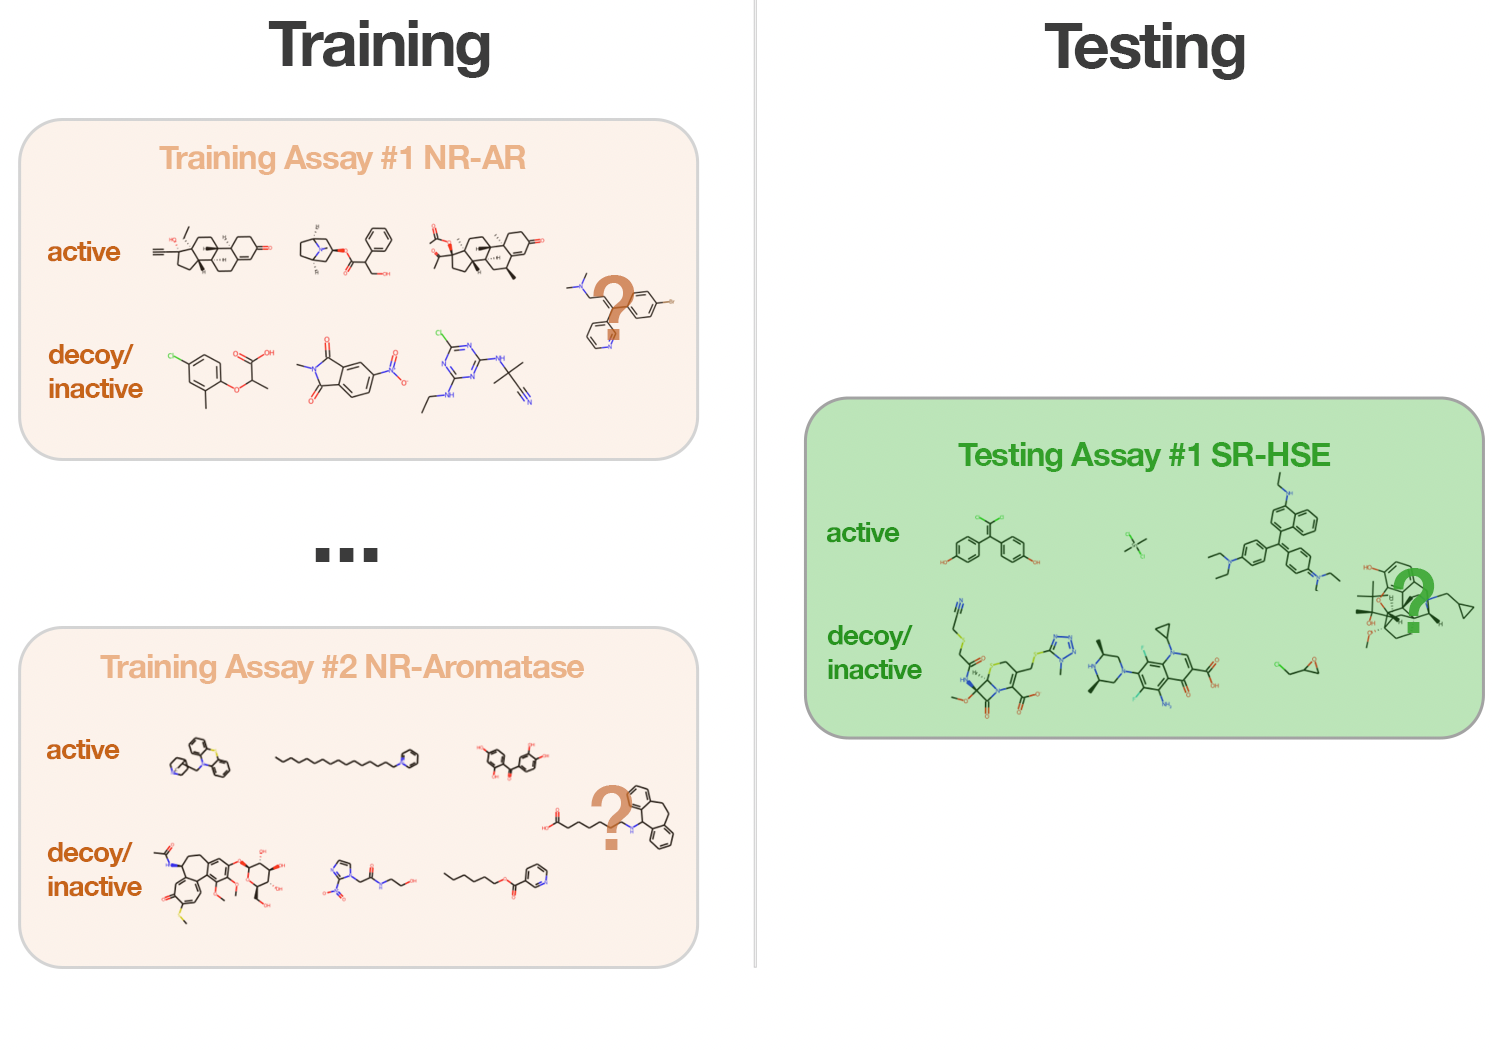
\includegraphics[width=0.8\linewidth]{img/tox21-metalearning.png}
	\caption{2-way 3-shot few-shot classification. Training a meta-learner on a set of experimental assays, and generalising for an unseen assay in the Tox-21 dataset.}
	\label{fig:tox21metalearning}
\end{figure}

Building on this notion, we aim to explore few-shot learning for virtual screening to address the low-data problem in this domain. The ability for a machine learning model to learn new concepts fast with just a few training examples is invaluable for virtual screening, where data on active compounds is scarce. Meta-learning aims to achieve generalising capabilities for environments that were previously unseen during training time. In meta-learning, such as few-shot classification, we train using a variety of training tasks and optimise for performance over a distribution of tasks, including unseen ones. Learning consists of a series of episodes, each consisting of an \textit{N}-way \textit{K}-shot classification task, effectively simulating the conditions at testing time. The \textit{way} refers to the number of classes we have per task and the number of samples we have is the \textit{shot} component. These samples make up the support set \cite{snell2017prototypical}. During test time, a small support set is sampled from new, previously unseen targets, and these few data points are used by the model to generalise for the activity of query molecules against this new target \cite{vinyals2016matching}. Figure~\ref{fig:tox21metalearning} shows an example of a typical meta-learning scenario on the Tox21 dataset, where data from a set of training assays are used to train a model, which is in turn used to generalise for a new, unseen assay using a support set from this new assay. We highlight that few-shot learning in the domain under study is in contrast to other domains such as computer vision, where the trained model recognises new classes. For example, given a few images of a lion as the support set, the model must generalise for new unseen images of a lion. In this domain, the challenge is to generalise to the behaviour of molecules in experimental assays which are related but not identical to the assays in the training collection. Given a few molecules from new experimental assays, can the model predict the activity of molecules in this new assay?

\section{Related Work}

Inspired by human learning \cite{lake2015human}, few-shot learning makes use of data from similar tasks to compensate for the lack of data for the task at hand. Several successful research undertakings have exploited this paradigm \cite{koch2015siamese, vinyals2016matching, snell2017prototypical, sung2018learning}, mainly for the computer vision domain. Meta-learning refers to this ability to learn how to learn \cite{thrun2012learning, finn2017model}. Being able to learn from only a few examples is important as certain domains do not have access to the plethora of data that we see in other domains such as computer vision. This inaccessibility could be due to privacy, safety, or ethical issues. For instance, data acquisition can be problematic in the drug-discovery domain due to possible toxicity, low activity or solubility in clinical candidates. Learning with low data leads to less expensive data gathering and reduced computational cost for learning \cite{wang2020generalizing}.

\citet{altae2017low} introduce a deep-learning architecture for few-shot learning in drug discovery, building on past work in metric-based meta-learning \cite{vinyals2016matching}, in which they propose the iterative refinement long short-term memory (IterRefLSTM). IterRefLSTM builds on the Matching Networks \cite{vinyals2016matching} by introducing iterative refinement of embeddings using long-short term memory (LSTM) networks. We build on their work by applying other successful few-shot learning approaches to this problem domain. In this study, we explore the application of a number of few-shot learning architectures including, in chronological order, Siamese networks \citep{koch2015siamese}, Matching Networks \citep{vinyals2016matching}, Prototypical Networks \citep{snell2017prototypical} and Relation Networks \citep{sung2018learning}. This group of architectures fall under the umbrella of metric-based meta-learning. In our study, we embed molecule representations using graph convolution networks, and then use or learn a distance function over these embeddings. Effectively, metric-based learners seek to learn a relationship between the input embeddings in the task space. For the purposes of this study, few-shot learning refers to training with as little as one example per class, to a maximum of 10 examples per class. Training with only one example per class is referred to as one-shot learning \citep{koch2015siamese, vinyals2016matching}.

\subsection{Graph Neural Networks}

Before processing the embeddings using few-shot machine learning architectures, the SMILES molecular representations need to be represented in computational space. \citet{wu2018moleculenet} report that graph-based models outperforms conventional machine learning models on the majority of datasets, suggesting that a learned embedding is advantageous over other molecular representations. Thus, we opt for graph learned molecular representations to embed the input molecules. Graphs are natural representations of molecules, where nodes and edges represent atoms and bonds, respectively. When representing molecules, the set of vertices \textit{V} intuitively refers to atoms within a molecule, while the set of edges \textit{E} refers to the bonds that connects two atoms together (see Equation~\ref{eq_graph}). Selected properties such as atomic number, atom type, charge, and valences, among others, can be encoded in the node feature vector.

\begin{equation}\label{eq_graph}
	\mathcal{G}=(\mathcal{V}, \mathcal{E})
\end{equation}

Graph neural networks can be used to learn molecular representations by applying convolutional operators and pooling layers on the molecular graphs \cite{jiang2021could}. Embeddings learned through neural networks afford the construction of automated features, rather than fixed fingerprints. Graph neural networks are effective in transforming small molecules into real-valued vector representations, which has been found to be a productive way of processing small molecules within deep neural networks \cite{gomez2018automatic}. \citet{duvenaud2015convolutional} report that using a differentiable method reduces collisions of substructures, and the fingerprint can be optimised to contain only relevant features. The fingerprint's interpretability is enhanced as this method captures activity and similarity of substructures.

% If the graph object is our input signal, we can apply a set of operators for the function we are attempting to learn. \citet{bronstein2021geometric} propose four key building blocks for deep learning on graphs, which include linear set equivariant layers, non-linear functions, local pooling layers and set invariant layers (see Figure \ref{fig:graphlayers}). For graphs, the nodes $v$ are found on a domain $\Omega$ such that $v \in \Omega$. The nodes in $\Omega$ are stored in a feature space $C$, such that $C = \mathbb{R}^k$. Using a set of feature functions $X(\Omega, C)$, we can transform the feature space of the nodes in our domain. In the equivariant layer $B$, we can take the nodes in our domain and apply a function that transforms the features of the nodes such that $X(\Omega, C) \rightarrow X(\Omega', C')$. Equivariance allows for a function $g$ to be applied before or after this layer such that $B(g.x) = g.B(x)$. The non-linear activation functions can be applied element-wise on the features of the nodes in a graph, such that $(\sigma(x))(v) = \sigma(x(v))$. The invariant layer $Z$, which can also be referred to as a global pooling layer, in which $X(\Omega, C) \rightarrow y$, satisfies the invariant condition such that $Z(g.x) = Z(x)$ \citep{bronstein2021geometric}. 

% \begin{figure}
	%   \centering
	%   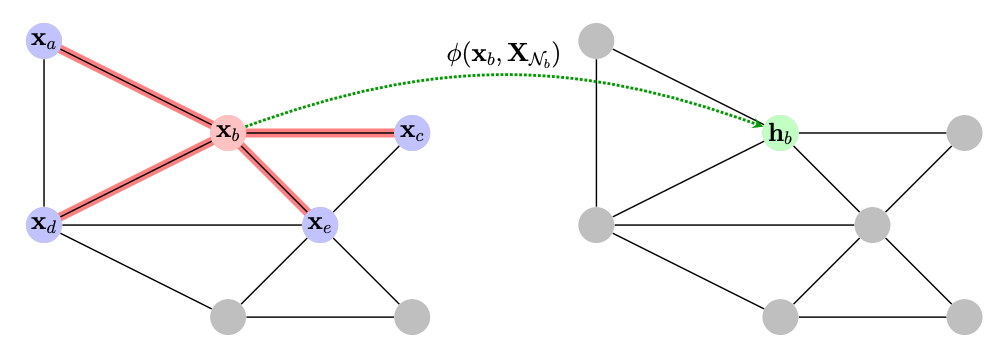
\includegraphics[width=0.9\linewidth]{img/conv-equivariance.png}
	%   \caption[Graph Convolution Function]{Equivariant function in a graph, synonymous with a graph convolutional operator over neighbouring nodes. Reproduced from \citet{bronstein2021geometric}.}
	%   \label{fig:convequivariance}
	% \end{figure}

% In Equation~\ref{gcnequation}, the current node is included in the aggregation of neighbouring nodes through the addition of the identity matrix to the adjacency matrix to form $\hat{A}$. The diagonal node degree matrix $D$ normalises $A$, the adjacency matrix, to preserve the scale of feature vectors, such that $D^{-1}A$, which is equivalent to averaging neighbouring node features. This is further enhanced through symmetric normalisation of $A$ through $D^{-1/2}AD^{-1/2}$, which gives us the propagation rule in Equation~\ref{gcnequation} \cite{kipf2016semi}. $W$ is the weight matrix for the $l$th layer, $H$ is a neural network layer and $\sigma$ is a non-linear activation function.

% \begin{equation}
	% \label{gcnequation}
	% f(H^{(l)}, A) = \sigma\left( \hat{D}^{-\frac{1}{2}}\hat{A}\hat{D}^{-\frac{1}{2}}H^{(l)}W^{(l)}\right)
	% \end{equation}
% where
% \begin{conditions*}
	%     A & Adjacency matrix \\ 
	%     $\hat{A}$ & $A + I$, in which $I$ is the identity matrix to include self-loops \\
	%     $\hat{D}$ & diagonal node degree matrix of $\hat{A}$ \\
	%     $\sigma(\cdot)$ & non-linear activation function \\
	%     W & weight matrix for the $l$ th layer \\
	%     H & neural network layer \\
	%     f & non-linear function \\
	% \end{conditions*}

% where
% \begin{conditions*}
	%     h_j & feature size of nodes \\
	%     N_i & set of neighbouring nodes i \\
	%     c_ji & product of the square root of node degrees \\
	%     b & learnable bias \\
	%     $\sigma$ & non-linear activation function \\
	% \end{conditions*}


% We then use a permutation-invariant global pooling layer, also referred to as a readout layer in literature \citep{wu2020comprehensive}. The readout layer is used to generate graph-level representations after the node features have been transformed using convolutional and local pooling layers. The readout layer is typically used at the end of the \ac{GNN} pipeline as the node representations are collapsed into a vector representing the graph \citep{wu2020comprehensive}. This vector can be further processed by multilayer perceptrons (MLP) to classify the final output, as shown in Figure \ref{fig:graphconvnetwork}.

\subsection{Metric-based few-shot learning}

The success of a few-shot learning model for metric-based meta-learning is dependent on the effectiveness of the kernel $k_\theta$, which measures the similarity between data samples (see Equation \ref{kernel}) using a metric or distance function. The models discussed in this section, excluding the benchmark model, use the support and query embeddings generated from the graph neural network to learn the kernel function.

\begin{equation}
	\label{kernel}
	P_\theta(y \vert \mathbf{x}, S) = \sum_{(\mathbf{x}_i, y_i) \in S} k_\theta(\mathbf{x}, \mathbf{x}_i)y_i
\end{equation}

\subsubsection{Siamese Networks}

Siamese networks \cite{bromley1993signature, koch2015siamese} are composed of two identical networks, with shared weights and parameters, taking in a pair of data samples as inputs. As the neural networks share weights, the feature extraction is maintained to the same feature space for both inputs. These identical subnetworks are finally connected in a final layer that acts as a distance function for the two outputs.

\subsubsection{Matching Networks}

Building on Siamese Networks, but instead of learning a metric function over pairs of data, the classifier learns how to define a probability distribution of output labels from query/test examples using a support set $S$ \cite{vinyals2016matching}. The classifier outputs a sum of attention weighted labels from the support set to predict the similarity between the test example and the samples from the support set. We use the same embedding function for the support and query sets to compute the molecular embeddings. Subsequently, the cosine similarity between pairs of data points between the support and query sets is computed, which is then normalised by a softmax function. The attention mechanism $a$ in $\hat{y} = \sum_{i=1}^{n} a(\hat{x}, x_i)y_i$ specifies how similar $\hat{x}$ is to each example $x$ in $S$.

\subsubsection{Prototypical Networks}

Proposed by \citet{snell2017prototypical}, these networks are similar to Matching Networks, but instead of comparing the query support to every support data point, a \textit{prototype} is calculated, which takes all the support data points per class and creates an embedding by averaging over the embeddings. The euclidean distance between the query data points and the prototypes is calculated for classification. In a one-shot learning scenario, Prototypical Networks are equivalent to Matching Networks, however, the Euclidean distance is used instead of the cosine distance used in Matching Networks.

\begin{figure}[h]
	\centering
	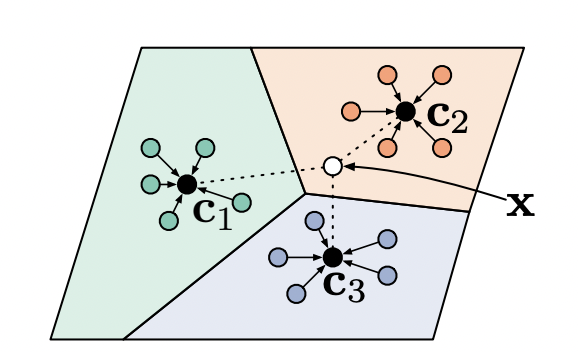
\includegraphics[width=0.7\linewidth]{img/protonets.png}
	\caption{Few-shot learning in Prototypical Networks, where prototypes \textbf{$c_k$} are taken as the mean of embedded support examples for each class. Reproduced from \citet{snell2017prototypical}.}
	\label{fig:protonets}
\end{figure}

\subsubsection{Relation Networks}

\citet{sung2018learning} present the Relation Network, a framework for few-shot learning, which could also be extended to zero-shot learning. The Relation Network learns a non-linear distance metric to compare support and query examples. As opposed to the aforementioned networks, this network uses a feed-forward neural network to learn a distance function in feature space. After embedding the support and query examples through an embedding function, each query example is concatenated with each of the feature maps. The resulting feature map concatenations are processed using a convolutional neural network to output a relation score vector, from which the class can be inferred.

\subsection{Iterative Refinement LSTM}

\citet{altae2017low} propose the iterative refinement long-short term memory (IterRefLSTM) to further process the resulting embeddings in a few-shot machine learning pipeline. In IterRefLSTMs two embedding functions $f(\dot|S)$ and $g(\dot|S)$ are developed simultaneously. Therefore, the embedding of the query is built iteratively with that of the support set, using information from both sets to enhance both the support and query embeddings (see Figure~\ref{fig:iterreflstm}).

\begin{figure}[h]
	\centering
	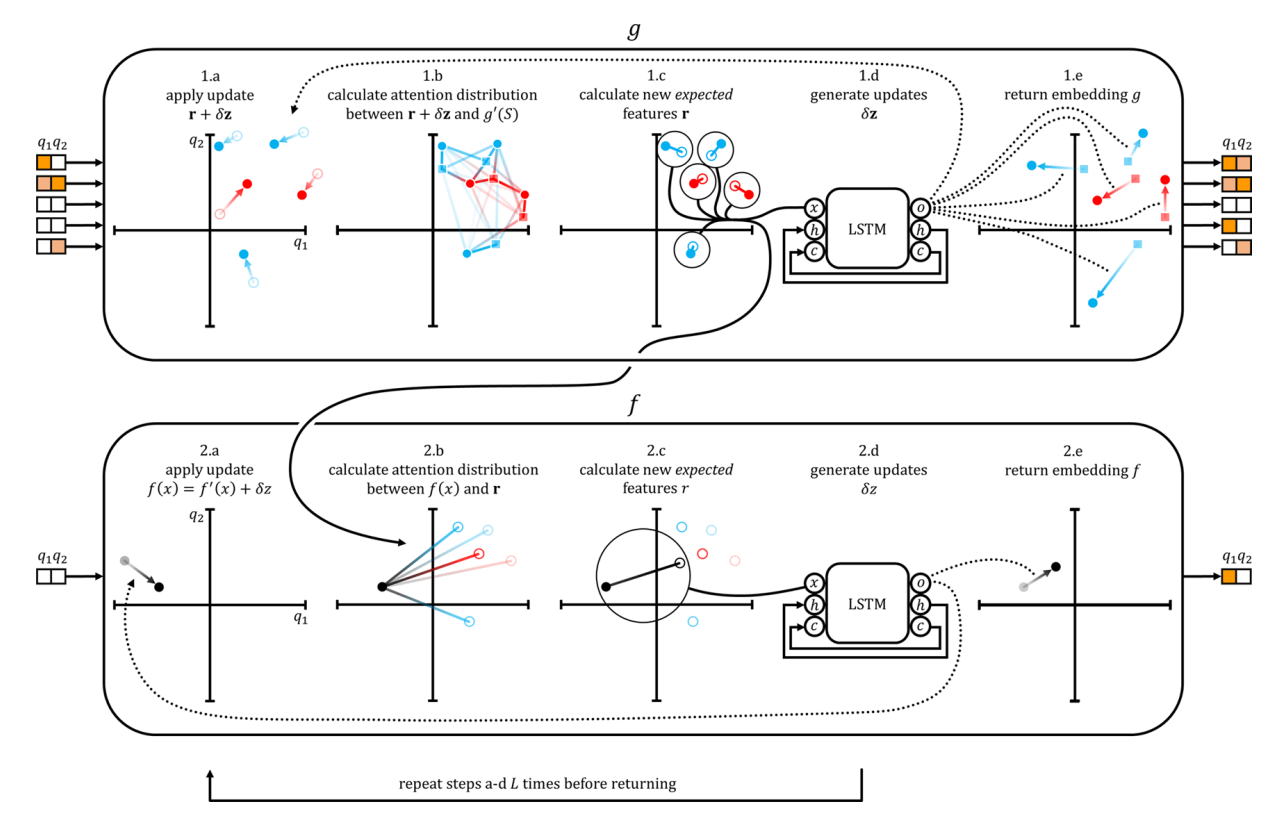
\includegraphics[width=\linewidth]{img/iterreflstm.png}
	\caption{Iterative refinement of embeddings using an LSTM network. The red and blue points depict the active and inactive/decoy class, respectively. The squares depict the original embedding from $g'$. Reproduced from \citet{altae2017low}.}
	\label{fig:iterreflstm}
\end{figure}
